%!TEX root = MemoireZelliges_simple.tex

\chapter{Problématique}
%======================================================================

L'architecture musulmane, et donc celle du Maroc, est intimement 
liée à la religion. Les premiers conquérants nomades n'étaient pas 
des bâtisseurs. Cependant la liturgie de l'Islam nécessite une 
architecture pour rassembler les fidèles lors de la prière commune du 
vendredi. À l'origine très rudimentaire, cette architecture va peu à 
peu s'enrichir au contact de celles, prestigieuses, des civilisations 
conquises. La \emph{mosquée du vendredi} (\emph{Masj'id-el-Djami}) 
qui réunit l'assemblée (\emph{Ouma}) n'est pas seulement un lieu de 
prière, c'est également là que l'on discute des affaires courantes. 
On peut donc dire qu'elle a un rôle particulièrement important dans 
la vie de la communauté.

C'est dans l'architecture, d'abord religieuse, que l'art islamique a 
trouvé l'un de ses lieux d'application privilégiés, l'autre étant le 
livre. Avec le développement des cités, les principes décoratifs 
inventés pour les mosquées ont été transposés dans l'architecture 
civile.

Le Maroc a développé une forme d'art tout à fait particulière : 
l'art des zelliges. Il s'agit d'un revêtement de mosaïque de 
céramique glaçurée, décorant à la fois les murs et les sols.

\begin{figure}[htb]
  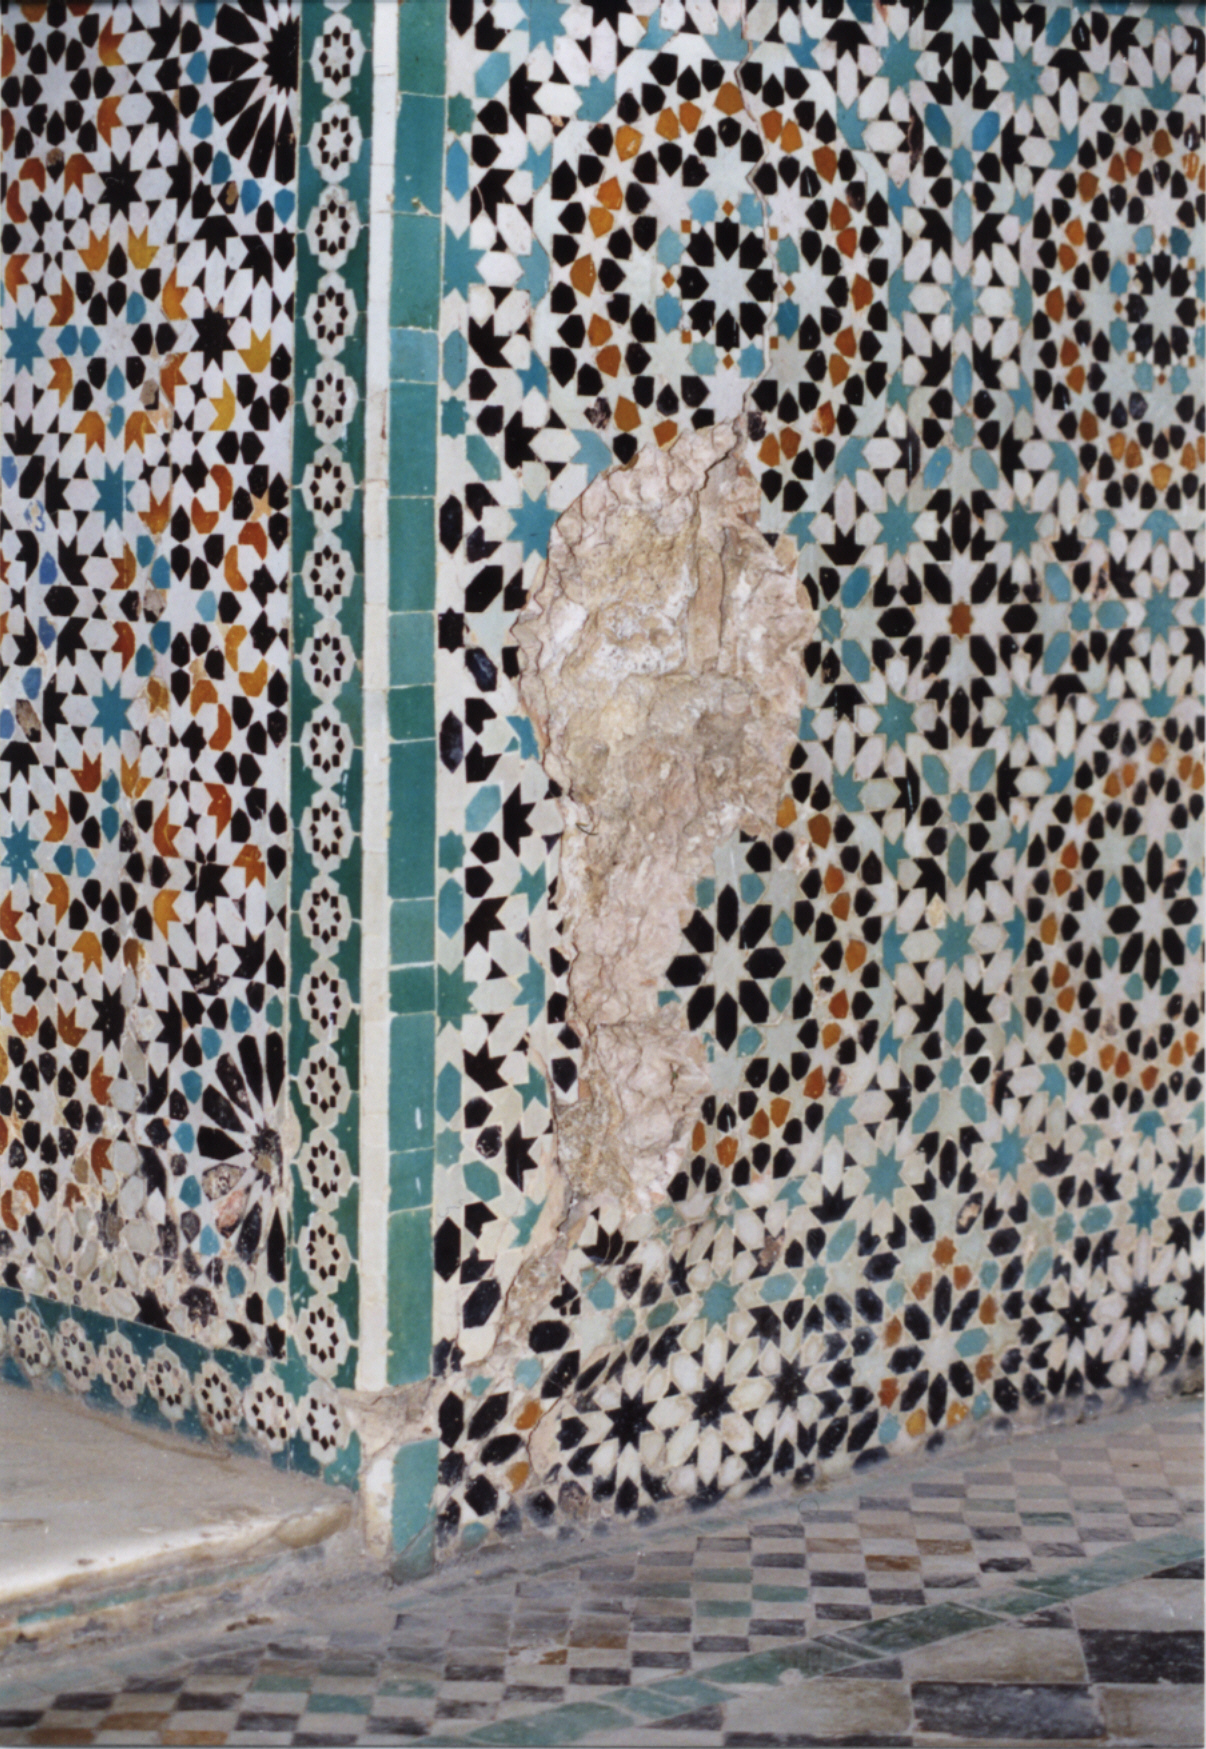
\includegraphics[width=0.45\textwidth]{alteration_1}%
  \quad%
  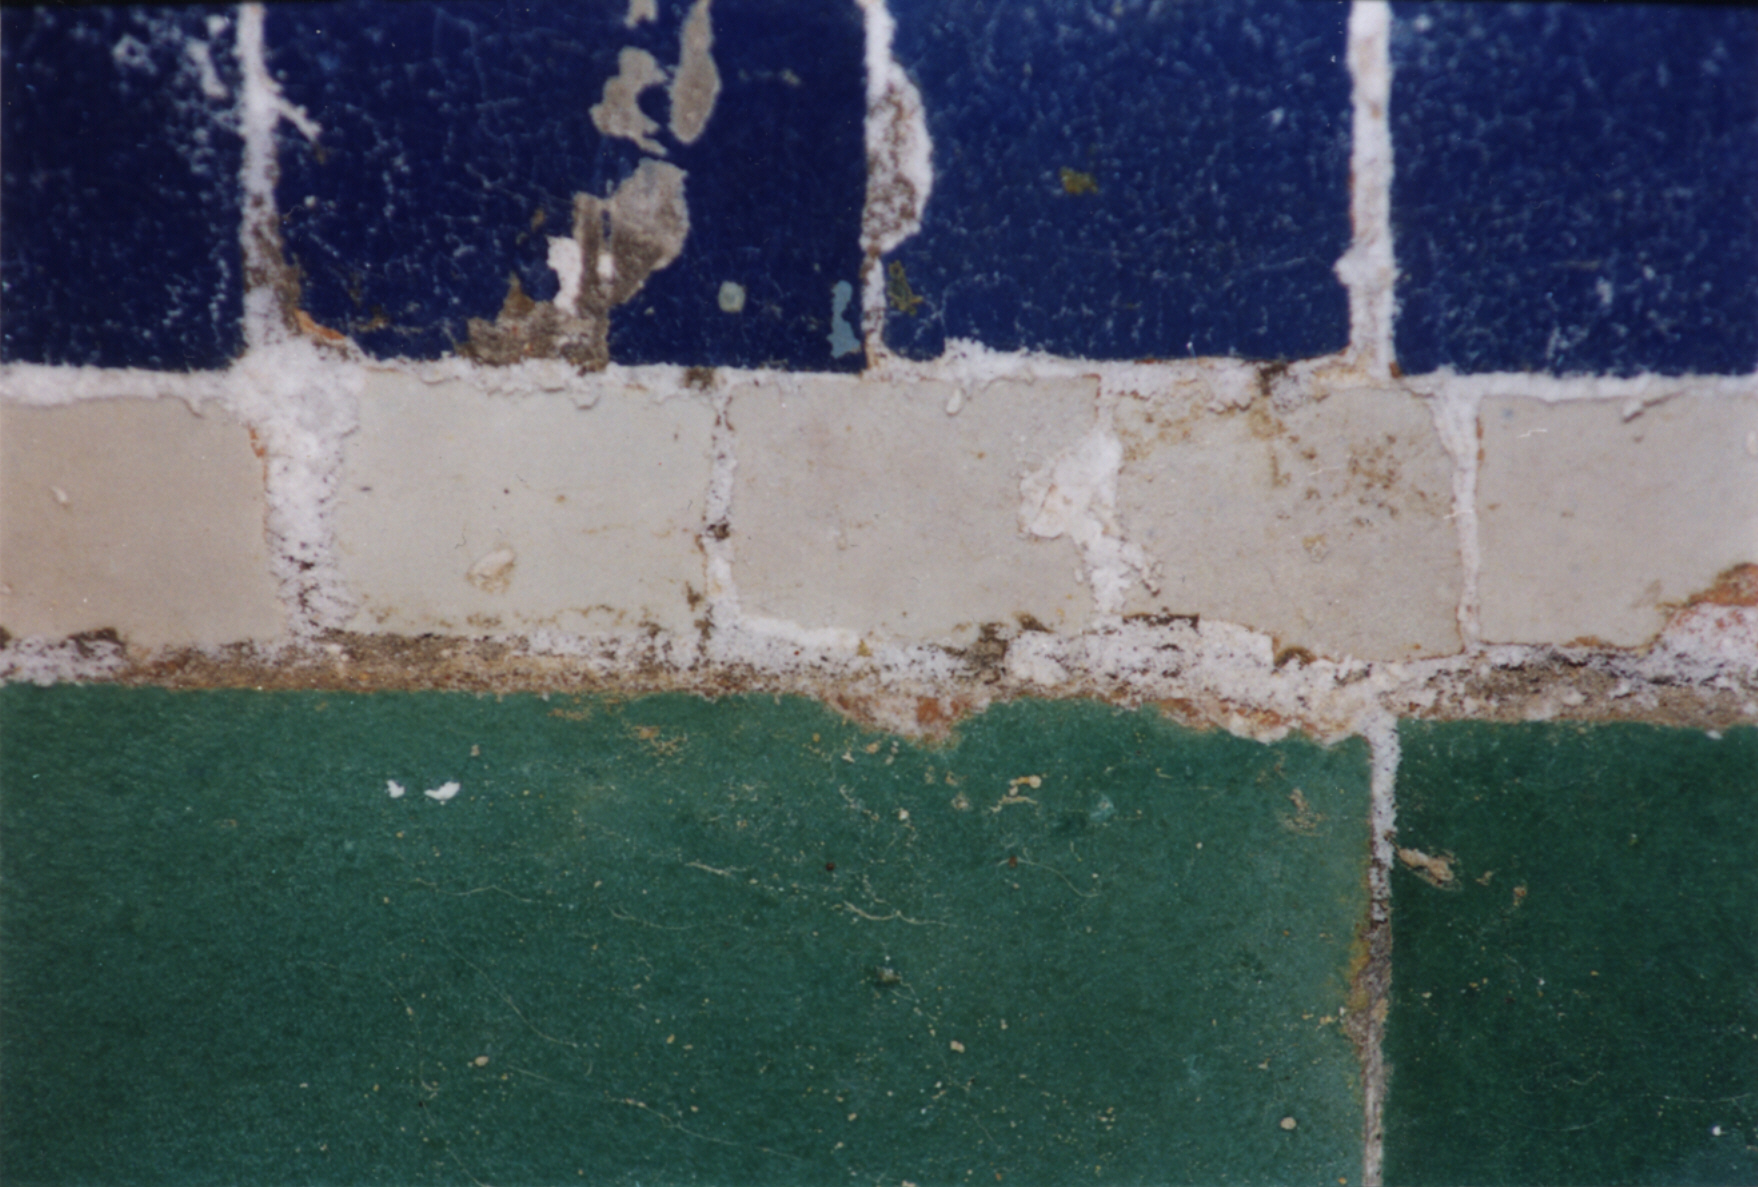
\includegraphics[width=0.45\textwidth]{alteration_2}
  \caption{Différents types d'altération : à gauche, on note un 
           décollement d'une partie du panneau décoré de zelliges ; 
           à droite, des efflorescences salines sont visibles entre 
           les pièces de céramique (clichés :~Schv{\oe}rer, 1999).}
  \label{fig:alteration}
\end{figure}

L'art des zelliges et les bâtiments qu'il décore font partie 
intégrante de la vie et du patrimoine culturel du Maroc. 
Malheureusement, ces témoignages du passé sont aujourd'hui 
victimes des ravages du temps : des panneaux entiers de zelliges 
se détachent, les glaçures sont altérées, on note également la 
présence d'efflorescences salines entre les pièces de céramique
(\fref{fig:alteration}).

Les architectes marocains souhaitent restaurer ces monuments et 
leurs décors de zelliges, en recréant les pièces manquantes selon 
les techniques anciennes, et dans la mesure du possible, mettre en 
{\oe}uvre une politique de conservation préventive. Mais ces 
techniques ne sont pas connues et les artisans actuels se sont 
adaptés aux matériaux modernes et colorants de synthèse.

La problématique de cette étude, portant sur les problèmes de 
préservation des céramiques glaçurées architecturales, s'articule 
donc autour de deux thèmes, dans le but de fournir aux architectes 
les données physico-chimiques nécessaires à leurs travaux : d'une 
part la recherche des techniques de fabrication anciennes, d'autre 
part l'évaluation et la caractérisation des phénomènes d'altération 
rencontrés dans ce type de matériaux.

\chapter{État des connaissances}
%======================================================================

\section{Zelliges}
%----------------------------------------------------------------------

\subsection{Définition}
%~~~~~~~~~~~~~~~~~~~~~~~~~~~~~~~~~~~~~~~~~~~~~~~~~~~~~~~~~~~~~~~~~~~~~~
On appelle \frquote{zellige} un art décoratif basé sur l'assemblage 
de pièces de céramique glaçurée chanfreinées, soigneusement 
découpées, puis assemblées de façon à former des motifs géométriques 
traditionnels. Ce terme désigne également les éléments de céramiques 
elles-mêmes. Les zelliges décorent aussi bien les murs que les sols, 
ou les colonnes des édifices religieux (mosquées, madrasas) et des 
demeures luxueuses.

Ce type de décor est réservé aux parties basses des murs, jusqu'à, 
à peu près, \SI{1.40}{\m} de hauteur. De cette façon, la frise de 
calligraphie, qui borde souvent la partie supérieure des panneaux 
de zelliges, est située à hauteur des yeux. La partie supérieure 
des murs est décorée de stuc sculpté, de boiseries.

Ce revêtement de zelliges est très important aux yeux des marocains 
et offre un contraste étonnant avec la terre battue et la poussière 
des ruelles extérieures. Afin de rester en permanence net et brillant, 
il a toujours fait l'objet des premiers soins de la journée. On 
rapporte que, jusqu'au début du siècle, le maître de maison venant du 
dehors avait coutume de quitter ses babouches au seuil de la cour, 
comme il l'aurait fait à l'entrée d'une mosquée.

\subsection{Historique}
%~~~~~~~~~~~~~~~~~~~~~~~~~~~~~~~~~~~~~~~~~~~~~~~~~~~~~~~~~~~~~~~~~~~~~~
L'origine de l'art des zelliges se situerait en \frquote{Orient}. 
Lors de la conquête du Maghreb et de l'Espagne pendant l'époque 
Omeyyade (\scl{viii}), les Arabes auraient amené avec eux de 
Syrie le principe du décor géométrique \autocite{Damluji_1993a}.

On trouve dans l'est du Maroc, sur des sites Fatimides et Hammadides 
des \sclnum{ix} et \siecle{xi}s (Tunisie et Algérie modernes), des 
décors fait de grands carreaux polychromes de céramique glaçurée, de 
forme géométrique (carreaux de pavement et de parement de la Qal'at 
Ban\=u Hammad). Ces mosaïques seraient inspirées de carreaux de 
céramique Aghlabides et abbassides (\sclnum{viii}-\scl{ix}). Ces 
premiers types de décors auraient ensuite évolué pour donner la 
forme la plus ancienne de zellige à proprement parler : celle des 
minarets almohades et des tours du Maghreb et d'Andalousie des
\sclnum{xii}-\siecle{xiii}s. On peut en voir des exemples 
\incise{motifs blancs et vert turquoise} sur les minarets de la 
Kutubiyya (Mosquée des Librairies) et de la mosquée de la Qasba à 
Marrakech \autocite{Damluji_1993a}.

Les zelliges tels qu'ils sont définis aujourd'hui \incise{très 
petits carreaux monochromes formant une composition polychrome de 
plus de deux couleurs} ne connaîtront de réel essor qu'à la fin du 
\sclnum{xiii} et au début du \siecle{xiv}. C'est sous les Mérinides, 
aux \sclnum{xiv}-\siecle{xv}s, que l'art des zelliges atteint son 
apogée, tant techniquement qu'artistiquement.

En Andalousie, l'industrie zellige sera à cette époque supplantée 
par des imitations peintes sur de grands carreaux polychromes et 
sur d'autres types de carreaux de mosaïque (à reflets métalliques, 
\emph{cuerda seca}, \emph{cuenca}, champlevé). Bien que de tels 
carreaux aient été importés au Maroc et probablement fabriqués 
localement, cette technique ne remplaça pas les zelliges dont la 
tradition sera perpétuée par les Saadiens puis les Alaouites jusqu'à 
nos jours, probablement grâce au repli sur lui-même qui caractérise 
le Maroc à partir du \siecle{xvi} et au conservatisme de sa société 
\autocite{Damluji_1993a}.

On sait peu de choses sur les évolutions stylistiques des zelliges 
à partir du \siecle{xvii}. Ces périodes n'ont, en effet, quasiment
pas été étudiées car elles sont souvent considérées comme la période 
de déclin de l'art des zelliges et donc sans intérêt pour la plupart 
des auteurs.

Certains auteurs \autocite{Castera_1996, Soustiel_1985} mettent en 
avant une seconde hypothèse sur l'origine de la technique zellige. 
Elle aurait été introduite au Maghreb par l'intermédiaire 
d'immigrants espagnols réfugiés en Tunisie pendant la Reconquista 
au \siecle{xiv}. On parle notamment d'un artisan nommé \emph{Qaçim
al-Zalidji} qui aurait donné son nom à cette technique. C'est de là 
que les zelliges auraient été importés au Maroc.

Il est intéressant de noter la ressemblance entre les zelliges 
marocains et les revêtements \emph{qâshânî}, mosaïques de céramique 
glaçurées présentant des motifs floraux, que l'on trouve en Orient, 
à Hérât (Afghanistan) par exemple. De même, le décor géométrique 
n'est pas une spécificité marocaine : au \siecle{xix}, les surfaces 
architecturales de tout l'empire musulman s'en sont couvertes. 
Cependant, l'association, au Maroc, de la technique de la mosaïque 
avec le principe du décor géométrique a aboutit à un véritable art 
abstrait, au sens noble du terme. De plus, sa grande technicité et 
ses qualités artistiques le rendent réellement unique.

\subsection{Technique de fabrication}
%~~~~~~~~~~~~~~~~~~~~~~~~~~~~~~~~~~~~~~~~~~~~~~~~~~~~~~~~~~~~~~~~~~~~~~
Le principal centre de production de zelliges dans le Maroc 
pré-colonial est Fès. Les zelliges présentent ailleurs au Maroc, 
à Meknès, Rabat, Marrakech, Salé, sont, soit importés de cette ville, 
soit produits localement selon sa tradition. Fès a produit depuis 
l'époque médiévale des {\oe}uvres de grande qualité. Il existe 
cependant un deuxième centre de production d'importance, caractérisé 
par une technique de fabrication différente de celle de Fès, du moins 
aux \sclnum{xix}-\siecle{xx}s : Tétouan.

La différence entre ces deux techniques est bien documentée à partir 
de la fin du \siecle{xx}. À Fès, de grands carreaux d'argile sont 
cuits, glaçurés, puis soumis à une seconde cuisson pour fixer le 
mélange glaçurant. Les \emph{f\=urmas} (formes des pièces zellige) 
y sont découpés. Si la technique de Tétouan requiert également deux 
cuissons, les pièces de zelliges sont découpées dans les grands 
carreaux d'argile avant la première. La technique de Fès permet un 
meilleur ajustement des pièces entre elles. En effet, les pièces 
découpées avant la cuisson subissent pendant celle-ci un retrait. 
Néanmoins, la technique de Tétouan est plus facile à mettre en 
{\oe}uvre et les glaçures, plus épaisses, ont la réputation de durer 
plus longtemps et de produire une surface en relief plus attrayante.

Les origines et le développement historique de ces deux techniques 
sont loin d'être clairs. Les premiers exemples de zelliges 
\incise{carreaux monochromes des minarets et tours almohades} furent 
de toute évidence découpés avant la cuisson, à cause de leur taille. 
En revanche, les motifs complexes développés au Maroc sous les 
Mérinides, ainsi qu'en Andalousie (époque nasride) et en Algérie 
(époque zayanide) ont requis l'utilisation de la technique, plus 
précise, de découpe après glaçure. L'apparition, à la fin du Moyen-Âge 
en Espagne, de la technique de découpe avant cuisson est associée un 
appauvrissement de la gamme de compositions de zelliges. Dans le 
Maghreb, cette dernière technique n'est relevée que dans les 
constructions médiévales de Tlemcen et à Tétouan 
\autocite{Erzini_1993a}.

Tétouan étant pratiquement une ville nouvelle, fondée vers 1484 
par des immigrants de Grenade, l'origine de sa technique différente 
pourrait se situer en Espagne musulmane. D'autre part, il semble 
qu'il y ait eu un appauvrissement similaire des compositions zelliges 
au Maroc au début de la période Alaouite et par conséquent, la 
technique de Tétouan pourrait être le résultat d'un déclin général 
\autocite{Erzini_1993b}.

La technique de fabrication actuelle de Fès peut être décomposée en 
différentes étapes.

Tout d'abord, l'argile de \frquote{terre} issue des gisements aux 
alentours de la ville est trempée dans de grands baquets d'eau 
(\emph{zw\={a}b\={\i}}) jusqu'à ce qu'elle ramollisse. 
Elle fermente pendant vingt-quatre heures avant d'être travaillée. 
Le pétrissage amollit la pâte de sorte qu'elle peut être mise dans 
des moules de \SI{1}{\cm} de profondeur qu'on laisse ensuite au soleil 
pendant quatre heures pour que l'eau d'humidité s'évapore. 
Ce procédé, appelé \emph{tans\u{\i}f} ou \emph{ta\u{g}f\={\i}f}, est 
effectué en été et doit fournir un stock de carreaux bruts suffisant 
pour toute l'année. 
Lorsque l'argile est sèche, on procède à la découpe des carreaux de 
zellige à l'aide d'un outil métallique (\emph{al-q\={a}la}).

Une partie des carreaux est alors cuite alors que les autres 
(\emph{mzihr\={\i} nayy}) sont stockés jusqu'à ce qu'on en ait besoin.

Le mélange glaçurant est ensuite appliqué sur les carreaux cuits qui 
subiront une seconde cuisson.

Les couleurs primordiales sont le vert, le bleu, le miel, le blanc 
et le noir, auxquelles s'ajoutent le rouge et différentes nuances 
des couleurs de base. Les pigments proviennent de matériaux locaux.

Les deux cuissons sont menées dans le même four (\emph{far\={\i}na}). 
La partie inférieure du four est réservée aux carreaux séchés au 
soleil, alors que la seconde cuisson se déroule dans la partie 
supérieure. Chaque couleur nécessite une température de cuisson 
spécifique qui détermine sa position dans le four : le blanc et 
le bleu, exigeant une chaleur intense, sont placés tout en bas, le 
rouge et le jaune viennent ensuite, et enfin, on trouve le vert qui 
nécessite le moins de chaleur. Le feu est alimenté avec des noyaux 
d'olive concassés (grignon, déchets solides du broyage des olives).

Après les cuissons, vient le découpage des pièces de zellige 
(\fref{fig:procede_naqs}), à l'aide d'une herminette tranchante 
appelée \emph{manq\={a}\v{s}}. Ce procédé, appelé \emph{naq\v{s}}, 
est selon le \zlaygi (maître zelligeur) \d{H}assan bin 
al-\d{T}ayy\={\i}b al-Haytam\={\i} l'épine dorsale de l'art des 
zelliges, la base pour atteindre la précision.

\begin{figure}[htb]
  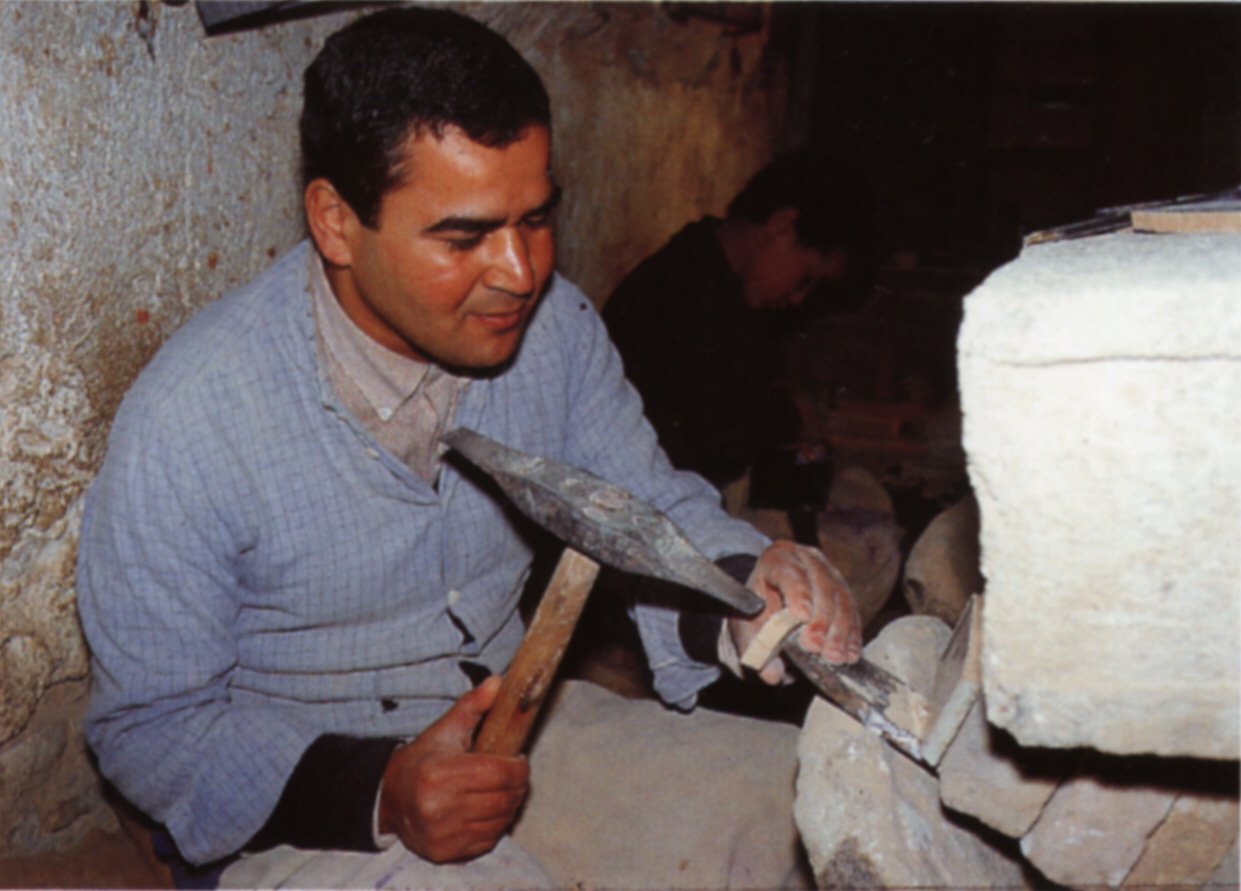
\includegraphics[scale=0.6]{procede_naqs_1}%
  \quad%
  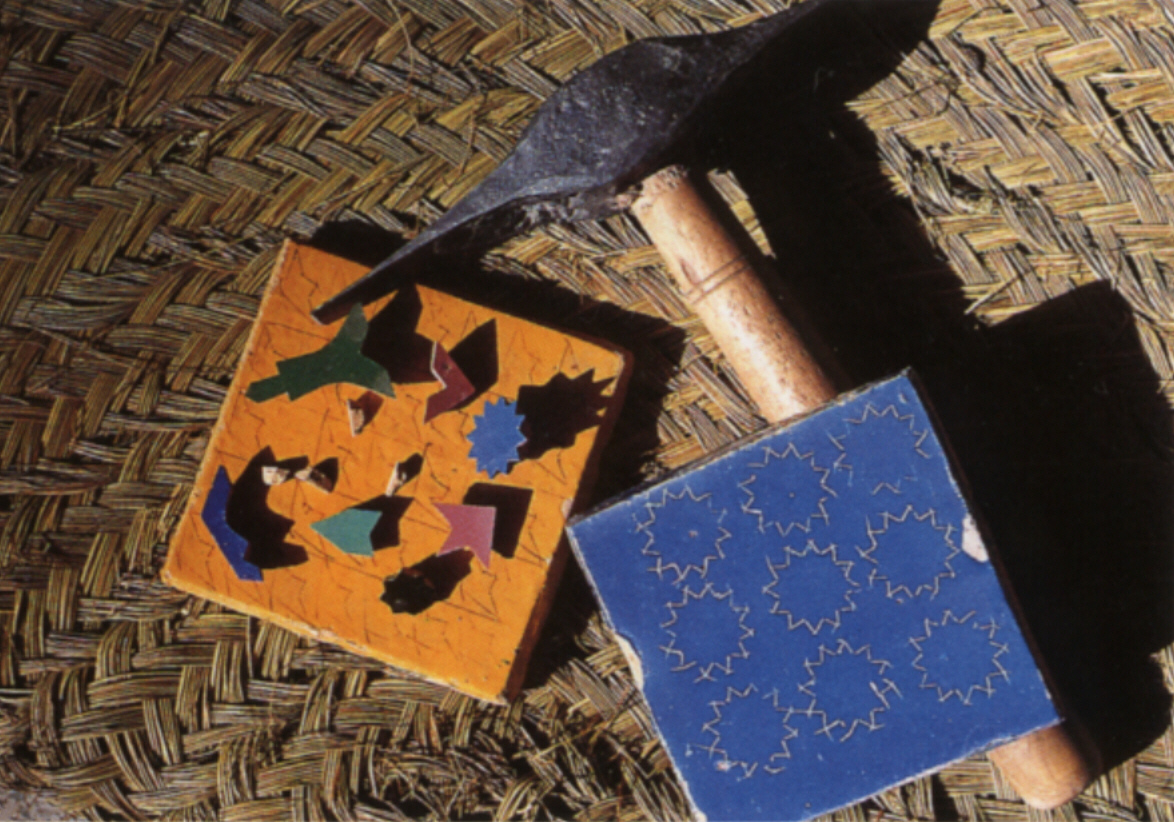
\includegraphics[scale=0.6]{procede_naqs_2}
  \caption[Procédé \emph{naq\v{s}} : découpage des pièces de zellige]
          {Procédé \emph{naq\v{s}} : découpage des pièces de zellige 
           \autocite{Castera_1996}}
  \label{fig:procede_naqs}
\end{figure}

La dernière étape est le \emph{far\v{s}} (\fref{fig:procede_fars}), 
\frquote{processus consistant à étaler les pièces 
\emph{zill\={\i}\u{g}} découpées devant derrière sur le sol selon 
l'agencement ou la composition du motif désigné en tant que partie 
de l'assemblage du panneau final}. \autocite{Damluji_1993a}.
Un premier mortier est utilisé pour souder les pièces entre elles. 
Une \emph{tafr\={\i}\v{s}a} (couche), de \SI{5}{\cm} de profondeur, 
d'un mélange de chaux et de sable est appliqué à l'arrière du panneau 
pour le fixer au mur.

\begin{figure}[htb]
  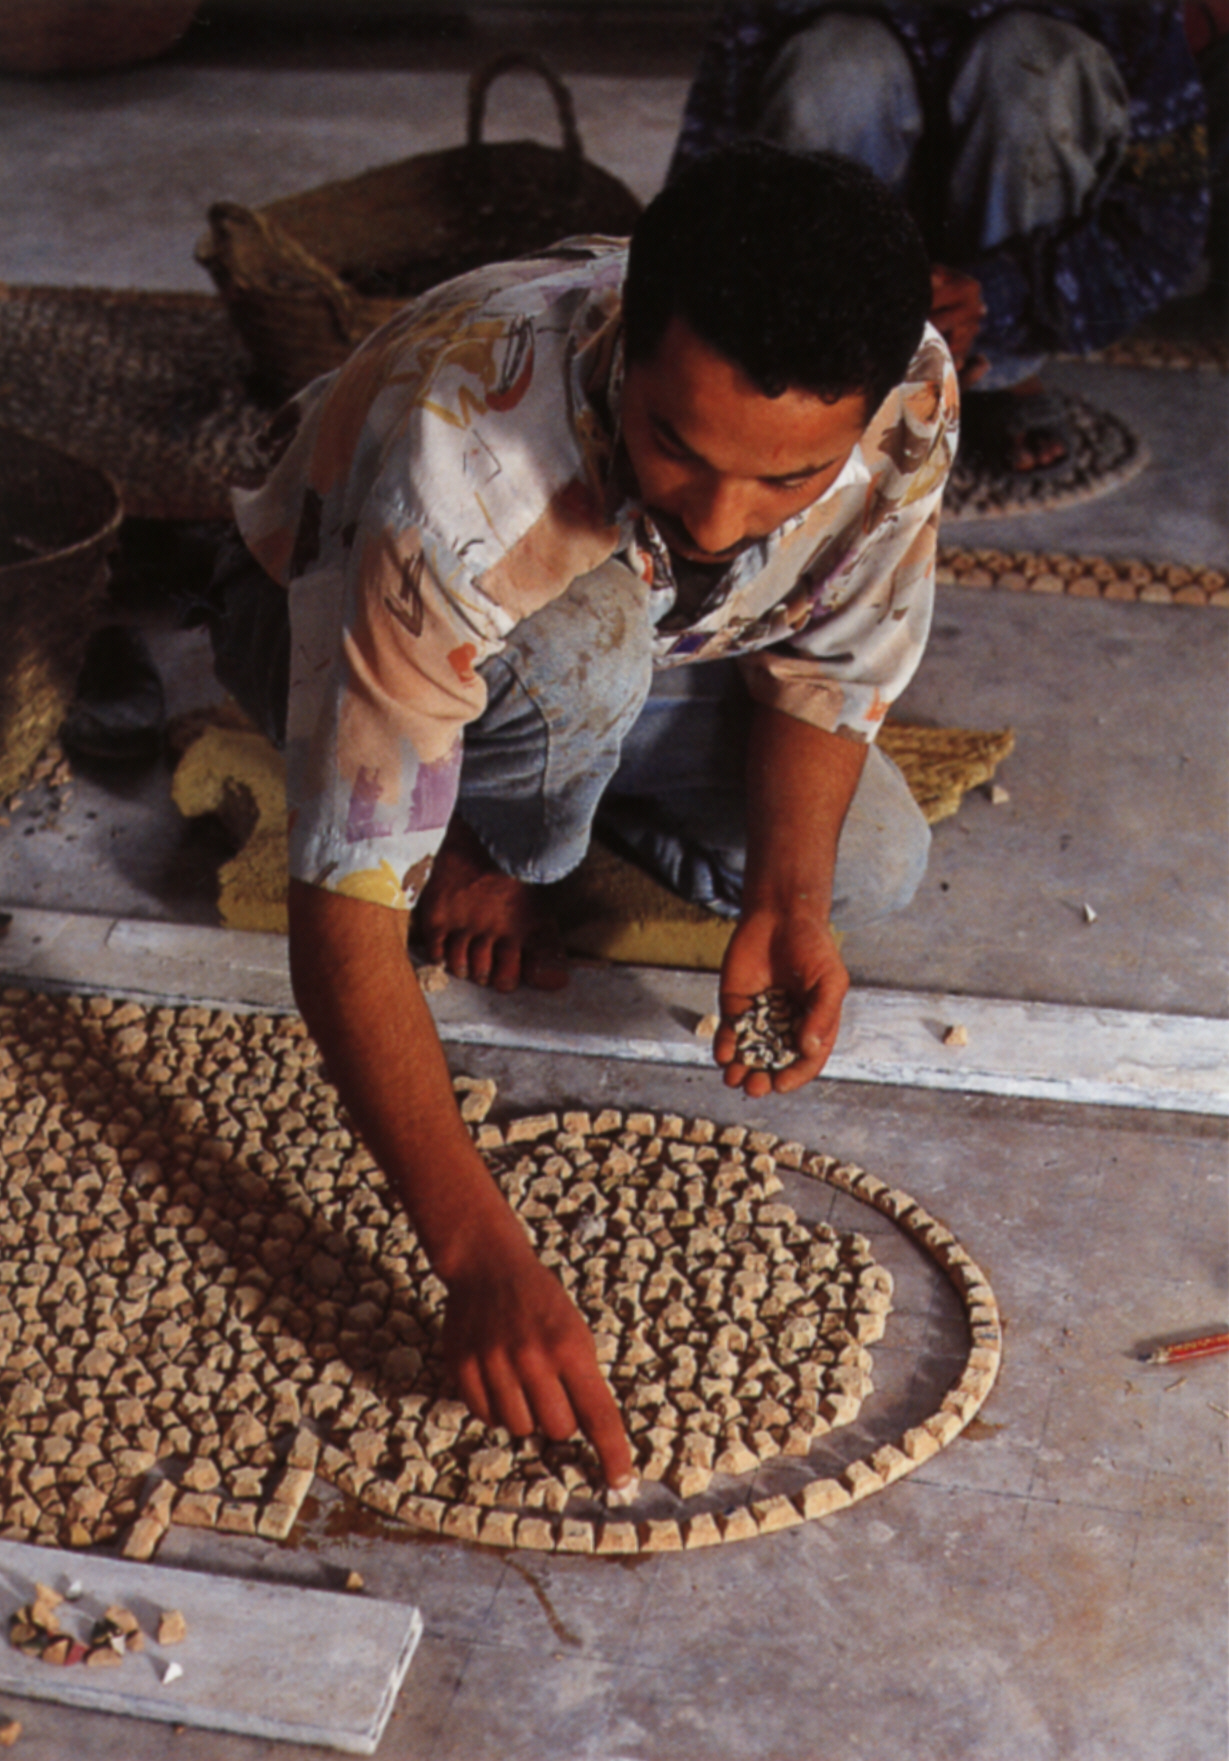
\includegraphics[scale=0.6]{procede_fars}%
  \caption{Procédé \emph{far\v{s}} : assemblage des pièces 
           \autocite{Castera_1996}.}
  \label{fig:procede_fars}
\end{figure}

% \begin{sidecaption}
%       [Procédé \emph{far\v{s}} : assemblage des pièces]
%       {Procédé \emph{far\v{s}} : assemblage des pièces 
%        \autocite{Castera_1996}.}
%       [fig:procede_fars]
%   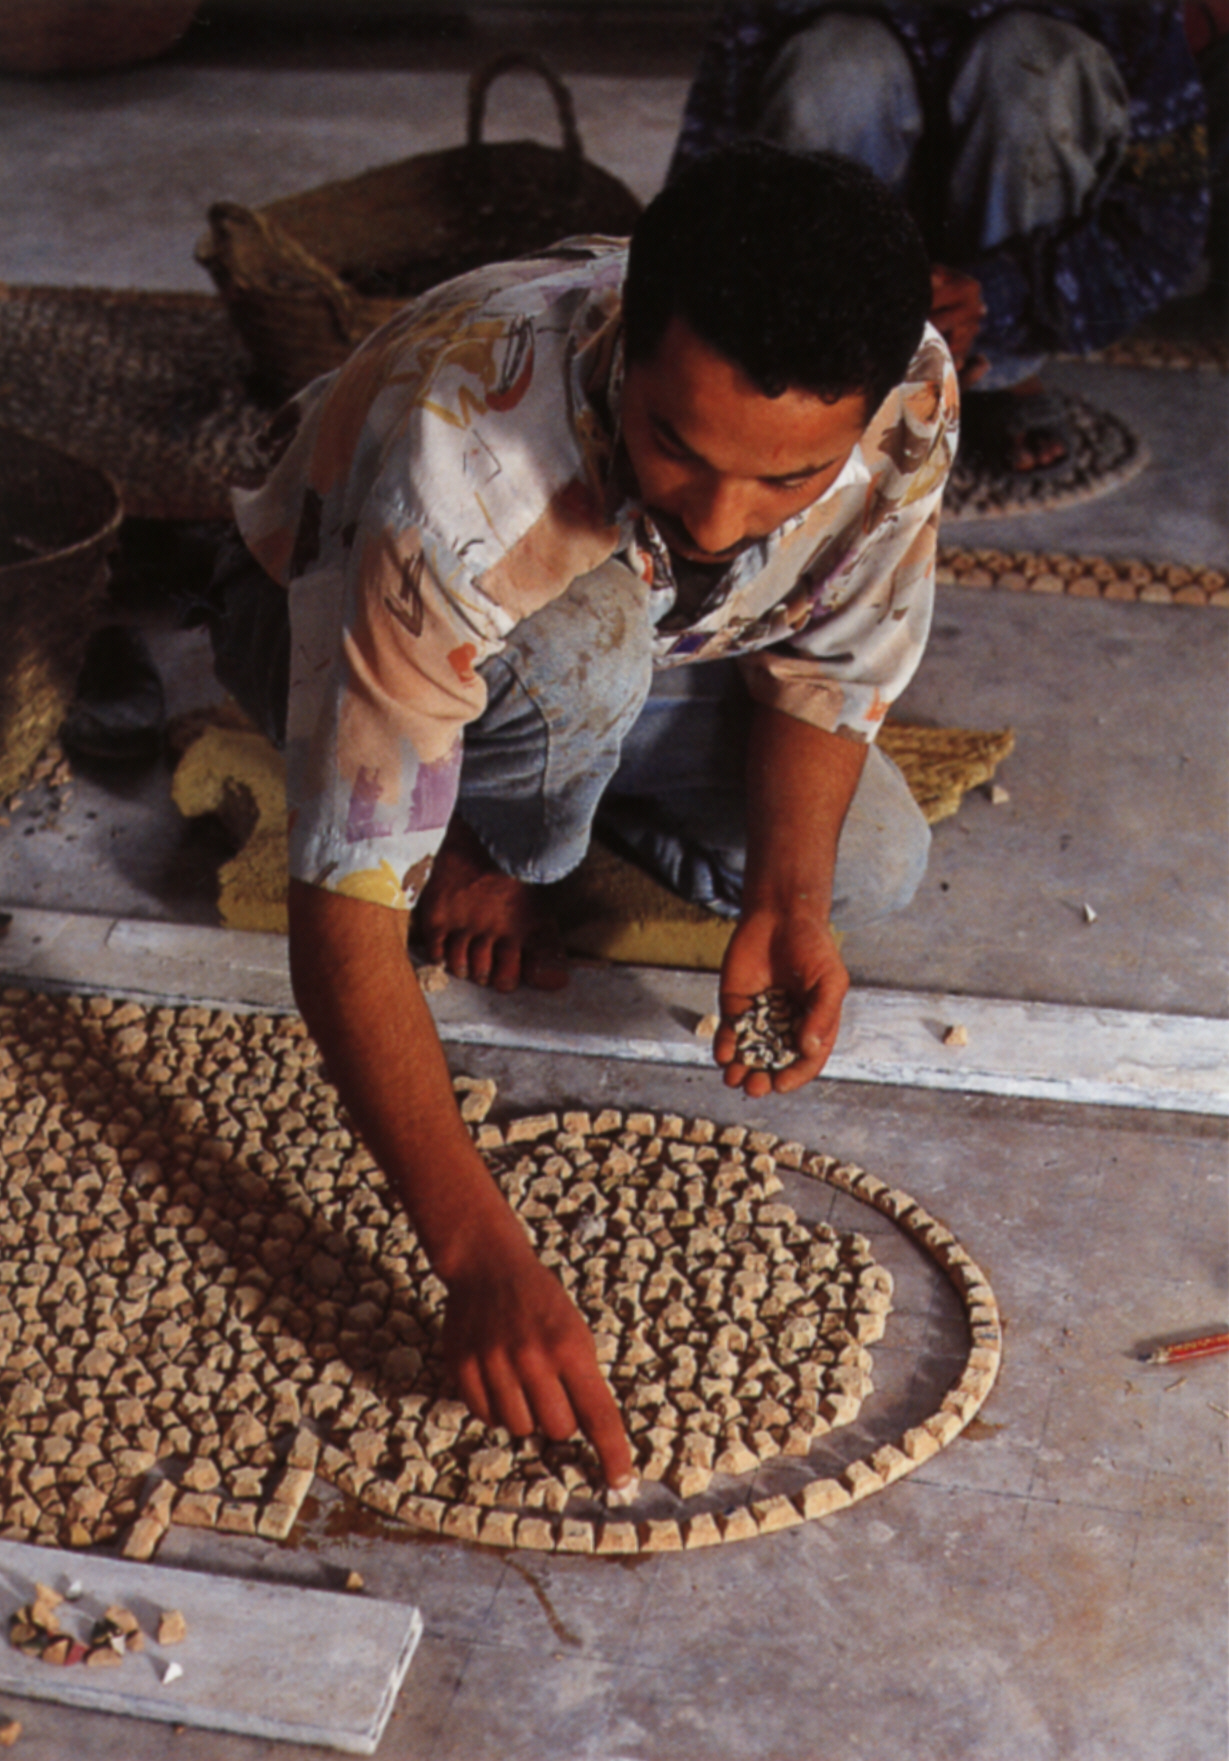
\includegraphics[scale=0.6]{procede_fars}%
% \end{sidecaption}

L'art des zelliges nécessite un apprentissage très long. Il faut 
passer par toutes les étapes du métier, des plus ingrates aux plus 
valorisantes, avant de devenir un \emph{maallem}, un maître-artisan. 
Al-Haytam\={\i}, soixante-cinq ans, est rentré dans le métier à l'âge 
de douze ans. Il passa d'abord sept ans comme apprenti, à dessiner 
les \emph{f\={u}rmas} et les compositions de zelliges, à apprendre 
le mesurage et les divisions géométriques qui leur sont liés. Il 
lui fallut vingt-et-un ans de plus pour maîtriser le découpage et 
l'équarrissage des pièces. Depuis, il se consacre à la fabrication 
de zelliges, au découpage et à la disposition des panneaux et à leur 
transport sur le site d'assemblage.

\subsection{Étude symbolique et géométrique}
%~~~~~~~~~~~~~~~~~~~~~~~~~~~~~~~~~~~~~~~~~~~~~~~~~~~~~~~~~~~~~~~~~~~~~~
Les trois genres de l'art islamique liés à l'architecture sont le 
décor calligraphique, l'arabesque florale et le décor géométrique. 
Toutes les écritures ont donné naissance à un art de la calligraphie. 
De même, des formes décoratives similaires à l'arabesque florale se 
sont développées dans d'autres civilisations : les enluminures 
moyenâgeuses ou les entrelacs celtiques par exemple. Le décor 
géométrique, en revanche, est une invention majeure de l'art 
islamique. Et c'est au Maroc et en Andalousie, à travers l'art des 
zelliges, que son développement fut le plus exceptionnel.

L'essor du décor géométrique est certainement lié à la limitation 
de la figuration imposée par la religion. En effet, si les images 
ne sont pas prohibées par le Coran, les \emph{Haddiths} 
\incise{commentaires ajoutés au Livre Saint au \siecle{ix}} 
proscrivent celles portant une ombre (statuaire, modelé en peinture, 
perspective). Ceci rendra possible le développement de la miniature 
aux \sclnum{xiii}-\siecle{xiv}s mais l'interdiction est totale dans 
les mosquées et les corans enluminés \autocite{Castera_1996}.

On peut rapprocher le décor géométrique islamique des traditions 
artistiques de sociétés primitives qui ont utilisé des symétries 
portant sur des formes géométriques simples. L'enracinement de l'art 
islamique dans ces formes et concepts archaïques lui donne une portée 
universelle. Son génie fut de développer un langage d'une richesse et 
d'une puissance d'expression extraordinaire. Dans ce type de décor, 
il n'y a plus de distinction fond-forme, les formes simples sont 
assemblées sans vide ni recouvrement. Seule la couleur impose au 
regard une interprétation plutôt qu'une autre \autocite{Castera_1996}.

L'art des zelliges est une image de la représentation islamique 
du monde. Il contient plusieurs niveaux de signification à la fois 
artistiques et scientifiques dont on ne peut saisir totalement le 
sens en quelques jours, quelques mois ou même quelques années d'étude.

Selon le \emph{maallem} A\d{h}mad D\={\i}b, seuls deux facteurs sont 
à prendre en compte pour comprendre cet art : d'une part, la pratique 
et la mémorisation du Livre Saint, base de son {\oe}uvre, de sa 
signification, de sa puissance ; d'autre part, la discipline 
d'apprentissage par c{\oe}ur qui est la base du talent visuel et 
manuel.

En fait, les maîtres-artisans pensent que leur art est une inspiration 
divine, Dieu est l'auteur suprême.

L'art des zelliges répond à certains principes de bases : les règles 
de proportions ne dépendent pas de codes empiriques traditionnels mais 
de nécessités purement géométriques ; le cadre arbitraire du motif ne 
doit être qu'une fenêtre ouverte sur un paysage abstrait qui reproduit 
à l'infini la même figure. La monotonie qui risquerait d'en découler 
est brisée par les imperfections résultant de la réalisation manuelle.

La \emph{f\={u}rma} de base est le \hatim (\fref{fig:furmas}), 
octogone étoilé ou sceau de Salomon. Toutes les autres 
\emph{f\={u}rma} en sont dérivées. Il est aussi le point de départ 
pour la division d'un motif et d'un panneau mural. Son axe est en 
quelque sorte le centre de gravité de la composition. Un \zlaygi 
confie : \frquote{Lorsque nous ajustons le positionnement du 
\emph{hamnisi} (motif étoilé à cinquante branches), nous nous servons 
du \emph{dabid} (compas à pointe sèche) pour produire un cercle 
parfait, en localisant le \hatim au centre : ceci nous donne la 
mesure, que ce soit un mètre ou deux, cent ou mille.} 
\autocite{Castera_1996}.

\begin{figure}[htb]
  \begin{tikzpicture}
    \node at ( 0.00, 0.00) 
          {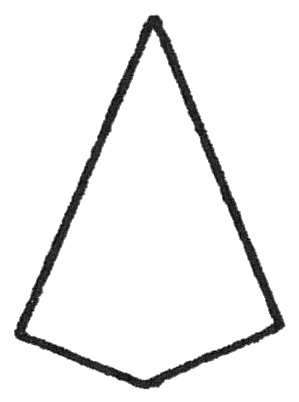
\includegraphics[scale=1]{furmas_luza}} ;
    \node at ( 0.00, 5.00) 
          {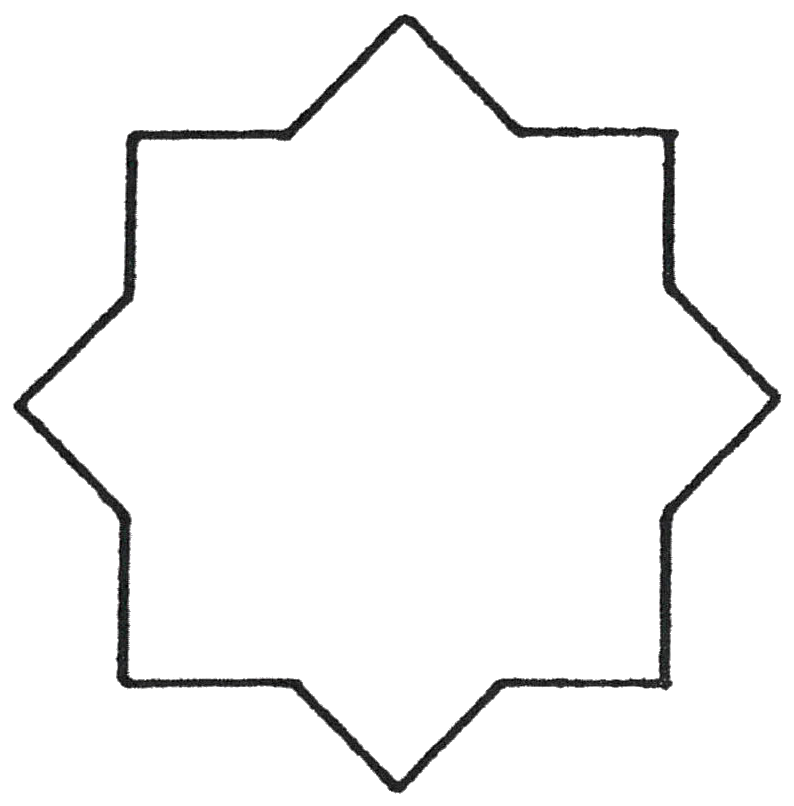
\includegraphics[scale=1]{furmas_hatim}} ;
    \node at (-3.00, 2.00) 
          {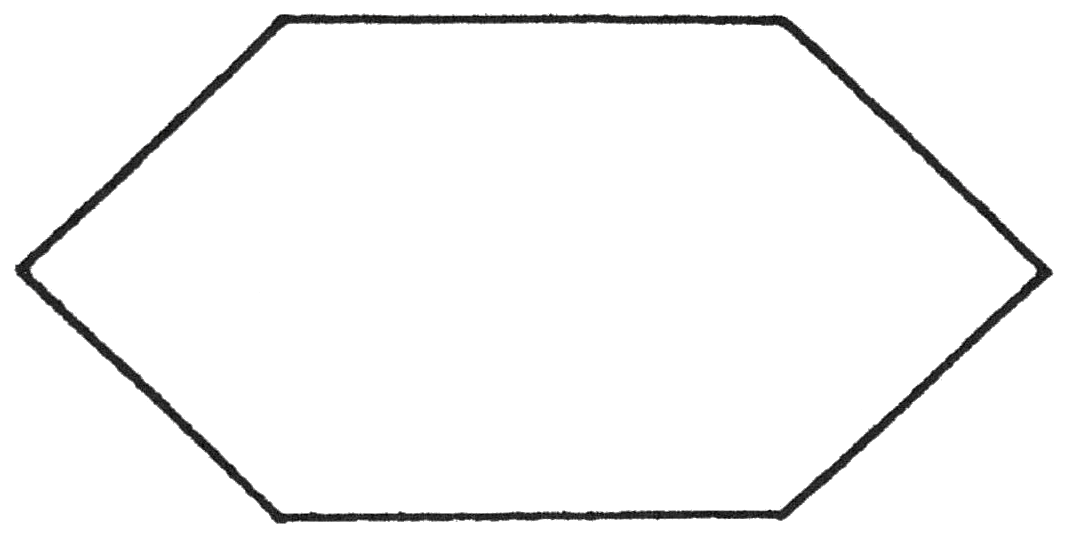
\includegraphics[scale=1]{furmas_saft}} ;
    \node at ( 3.00, 2.00) 
          {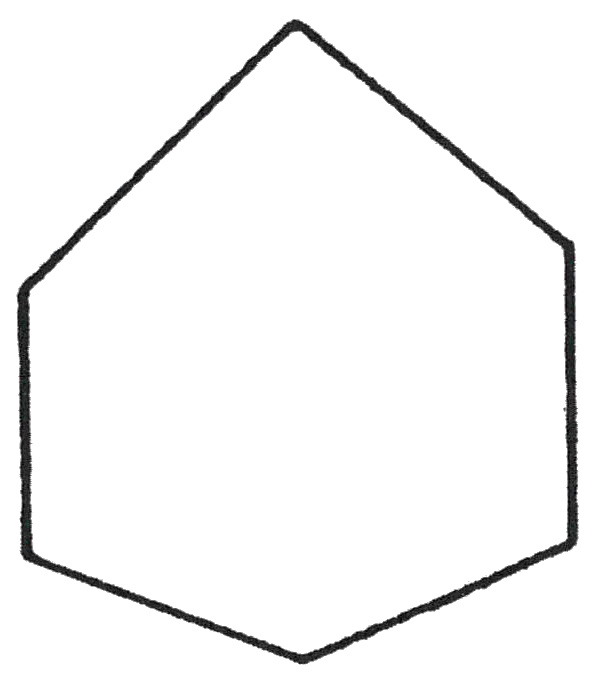
\includegraphics[scale=1]{furmas_kwayra}} ;
    \node at (-2.50,-2.00) 
          {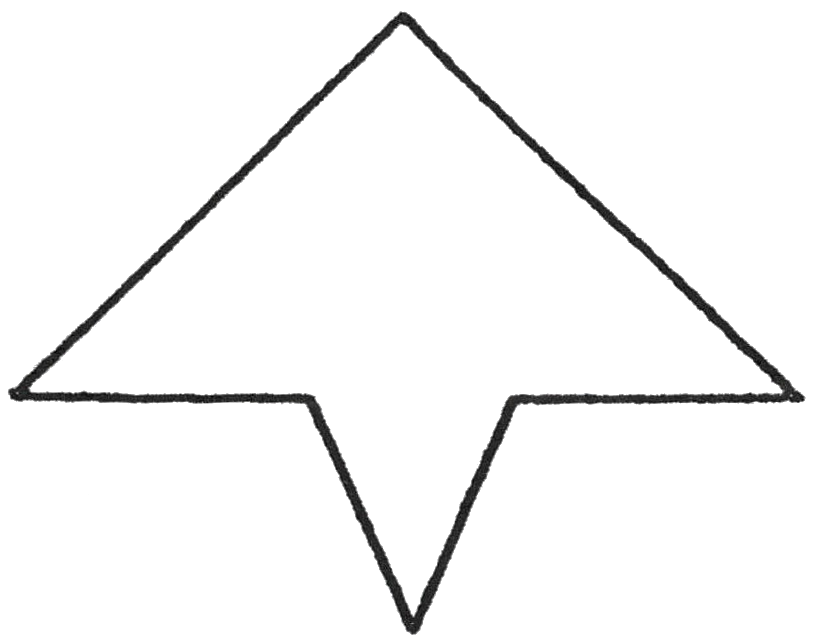
\includegraphics[scale=1]{furmas_hattayfa}} ;
    \node at ( 2.50,-2.00) 
          {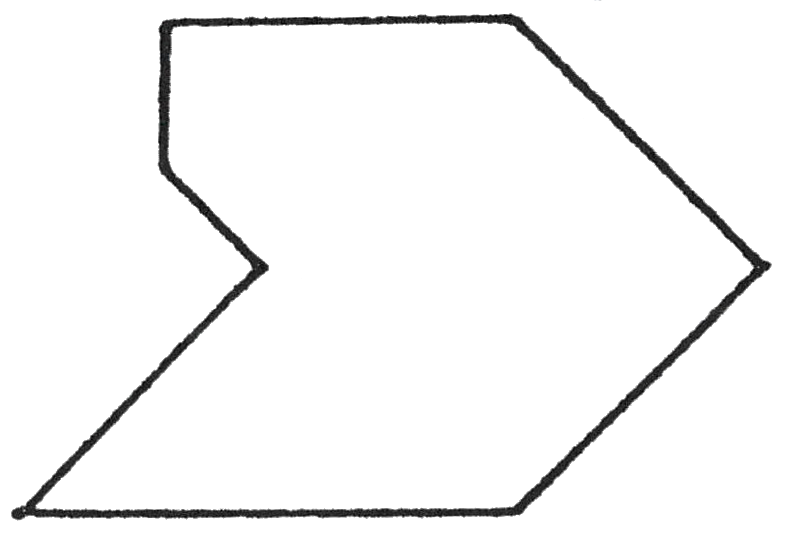
\includegraphics[scale=1]{furmas_fawrkat}} ;
  \end{tikzpicture}
  \caption{Différentes f\={u}rmas de zelliges \autocite{Castera_1996}.}
  \label{fig:furmas}
\end{figure}

Sa construction s'inscrit dans un cercle, forme parfaite par 
excellence, flanqué de quatre autres, tous identiques 
\fref{fig:cercle}. Cette figure symbolise pour Keith~\bsc{Critchlow} 
et Paul~\bsc{Marchant} les quatre coins du temps et de l'espace, à 
travers le cycle du soleil ou celui de la lune. Le cercle central 
représente le cycle complet et les quatre cercles adjacents sont 
l'image des quatre phases (solstices et équinoxes ou pleine lune, 
nouvelle lune, premier et dernier quartier).

\begin{figure}[htb]
  \begin{tikzpicture}[scale=2]
    \clip ( 0.00, 0.00) circle (2.3) ;

    \draw [dashed] ( 0.00, 0.00) circle (1) ;

    \draw [loosely dashdotted] plot(\x, \x) ;
    \draw [loosely dashdotted] plot(\x,-\x) ;
    \draw [loosely dashdotted] plot(\x,0) ;
    \draw [loosely dashdotted] plot(0,\x) ;

    \draw ( 1.00, 0.00) circle (1) ;
    \draw ( 0.00, 1.00) circle (1) ;
    \draw (-1.00, 0.00) circle (1) ;
    \draw ( 0.00,-1.00) circle (1) ;

    \draw [thick] \drawhatim ;
  \end{tikzpicture}
  \caption{Les cinq cercles dans lesquels s'inscrit le \hatim 
           \autocite{Castera_1996}.{}}
  \label{fig:cercle}
\end{figure}

On peut considérer que la plupart des motifs sont construits à 
partir de structures polygonales où alternent deux pièces 
essentielles, le \hatim et le \emph{\d{s}aft}. Une telle structure 
est le \frquote{squelette} (\fref{fig:squelette}) du motif qui 
apparaît quand les lignes courant vers l'intérieur se rejoignent 
en respectant les symétries de l'ensemble. On appelle cela la 
\frquote{résolution} du squelette On peut \frquote{déguiser} ces 
squelettes de sorte qu'ils ne soient pas directement discernables, 
ou même les éliminer totalement du motif. Les squelettes basés sur 
l'octogone sont les plus spécifiques du Maroc et les plus représentés 
dans son architecture. Ces squelettes, une fois habillés, sont 
associés en motifs périodiques. Comme la plupart des figures 
polygonales utilisées ne permettent pas de couvrir entièrement une 
surface plane, il faudra leur associer une ou plusieurs autres figures 
limitées par de nouveaux squelettes. De nouveaux motifs seront ainsi 
créés et ce processus est quasiment sans fin.

\begin{figure}[htb]

  \begin{minipage}[b]{0.33\textwidth}
    \centerfloat
    \begin{tikzpicture}[thick, fill=white, scale=0.4]
      \squelettea
      \fill (-2,-2) rectangle (2,2) ;
    \end{tikzpicture}
    \subcaption{\label{fig:squel_a1}}
  \end{minipage}%
  \quad
  \begin{minipage}[b]{0.33\textwidth}
    \centerfloat
    \begin{tikzpicture}[thick, fill=white, scale=0.4]
      \squelettea
      \filldraw \drawhatim ;
    \end{tikzpicture}
    \subcaption{\label{fig:squel_a2}}
  \end{minipage}%
  \quad
  \begin{minipage}[b]{0.33\textwidth}
    \centerfloat
    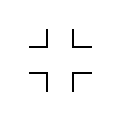
\begin{tikzpicture}[thick, fill=white, scale=0.4]
      \squelettea
      \fill (-1,-1) rectangle (1,1) ;
      \foreach \x in {0, 90, 180, 270} {%
        \draw [rotate=\x]
              ( {1-sqrt(2)} ,  1 )          -- 
              ( {1-sqrt(2)} , {sqrt(2)-1} ) -- 
              ( -1 , {sqrt(2)-1} ) ;
      }
    \end{tikzpicture}
    \subcaption{\label{fig:squel_a3}}
  \end{minipage}%

  \bigskip

  \begin{minipage}[b]{0.33\textwidth}
    \centerfloat
    \begin{tikzpicture}[thick, fill=white, scale=0.4]
      \squeletteb
      \fill (-0.5, 1) -- (-2.5,-1) -- 
            (0.5, -1) -- ( 2.5, 1) -- cycle ;
    \end{tikzpicture}%
    \subcaption{\label{fig:squel_b1}}
  \end{minipage}%
  \quad%
  \begin{minipage}[b]{0.33\textwidth}
    \centerfloat
    \begin{tikzpicture}[thick, fill=white, scale=0.4]
      \squeletteb
    \end{tikzpicture}
    \subcaption{\label{fig:squel_b2}}
  \end{minipage}%

  \caption{\subcaptionref{fig:squel_a1} et 
           \subcaptionref{fig:squel_b1} : différents squelettes ; 
           \subcaptionref{fig:squel_a2}, \subcaptionref{fig:squel_a3}, 
           \subcaptionref{fig:squel_b2} : diverses résolutions des 
           squelettes \autocite{Castera_1996}.}
  \label{fig:squelette}
\end{figure}

Les motifs de zelliges présentent des symétries intéressantes : on 
peut considérer un triangle minimal de base (\fref{fig:sym_triangle}) 
qui permet, par des symétries axiales (\fref{fig:sym_triangle} et 
\fref{fig:sym_dessin}) de reconstituer l'ensemble du motif 
(\fref{fig:sym_complet}).


\begin{figure}[htb]
  \begin{minipage}[b]{0.45\textwidth}
    \centerfloat
    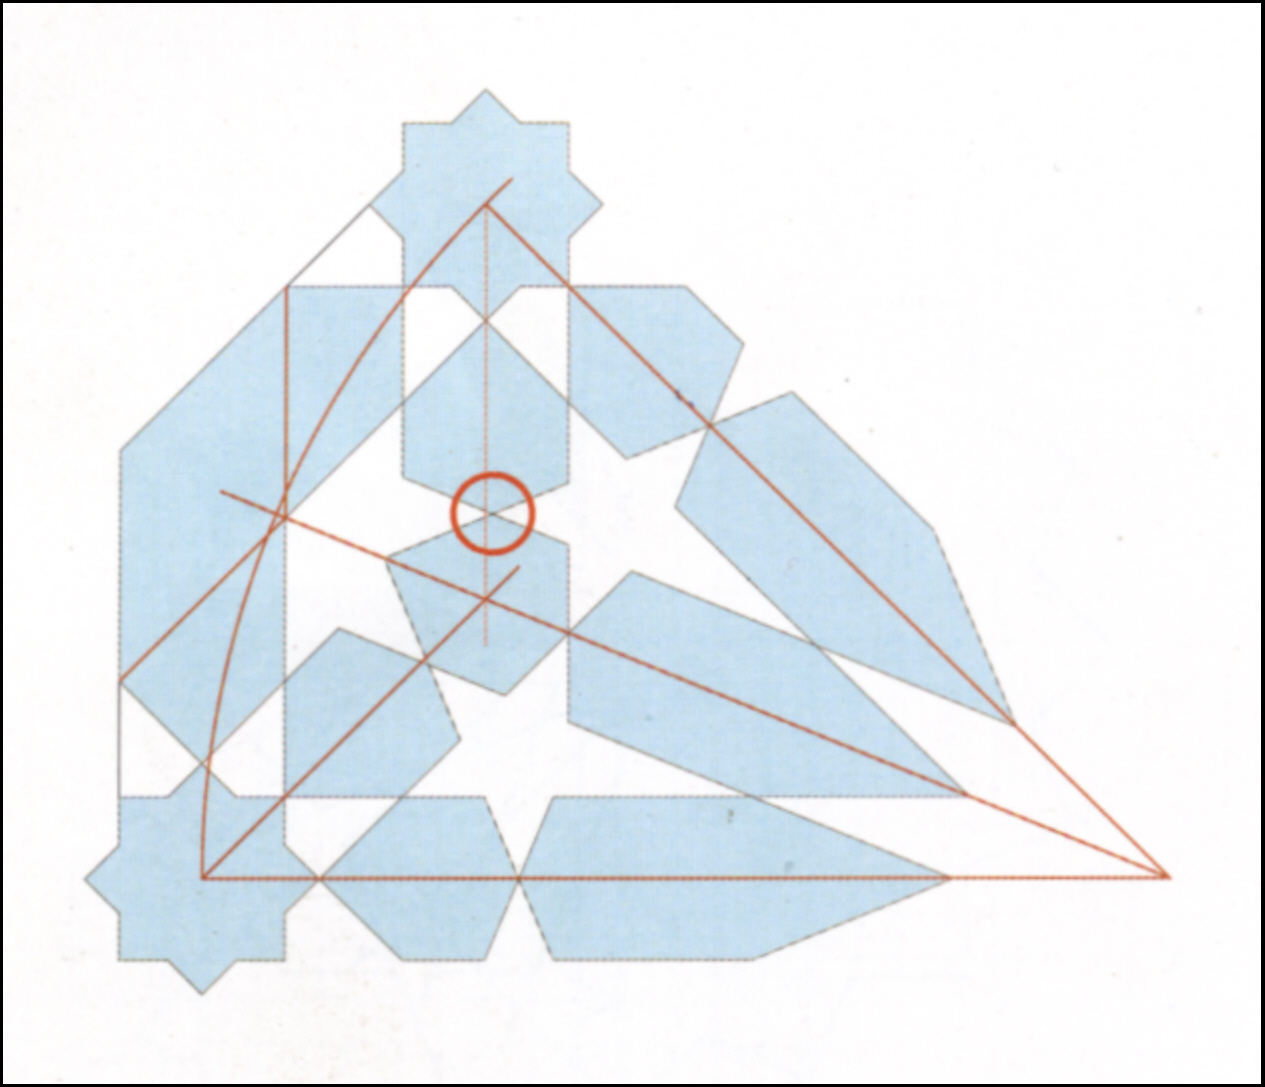
\includegraphics[width=\textwidth]{symetrie_motif_base_ori}
    \subcaption{Triangle minimal 
                \label{fig:sym_triangle}}
  \end{minipage}%

  \bigskip

  \begin{minipage}[b]{0.45\textwidth}
    \centerfloat
    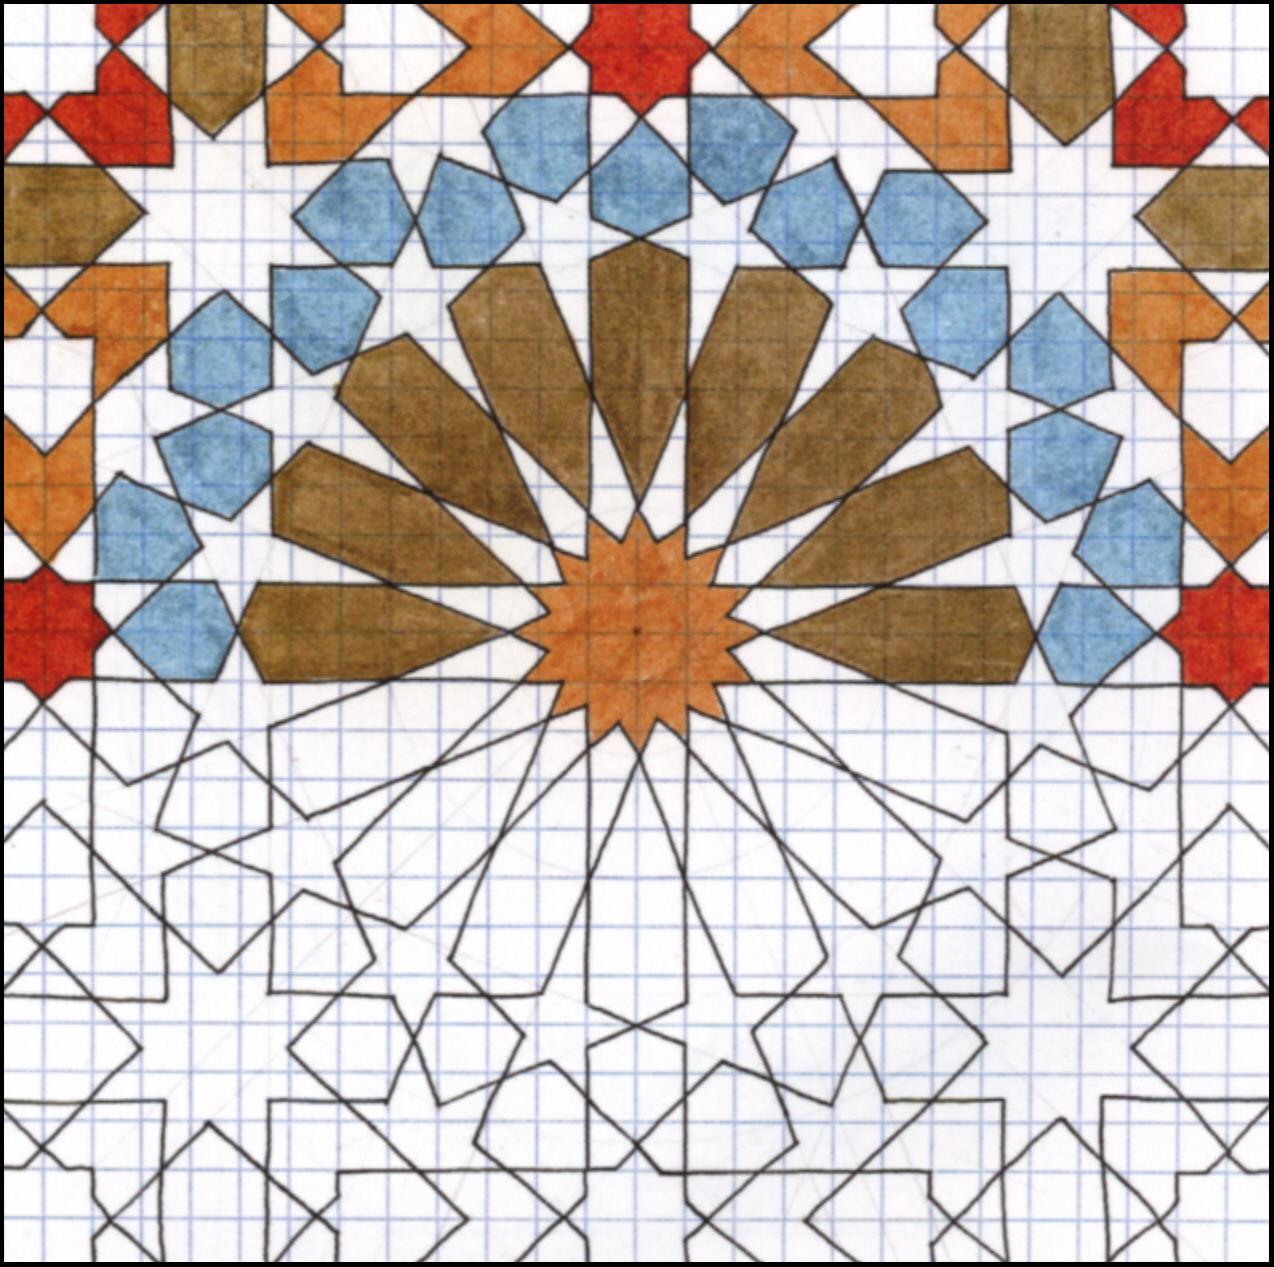
\includegraphics[width=\textwidth]{symetrie_motif_dessin}
    \subcaption{Construction du motif par symétries 
                \label{fig:sym_dessin}}
  \end{minipage}%
  \quad
  \begin{minipage}[b]{0.45\textwidth}
    \centerfloat
    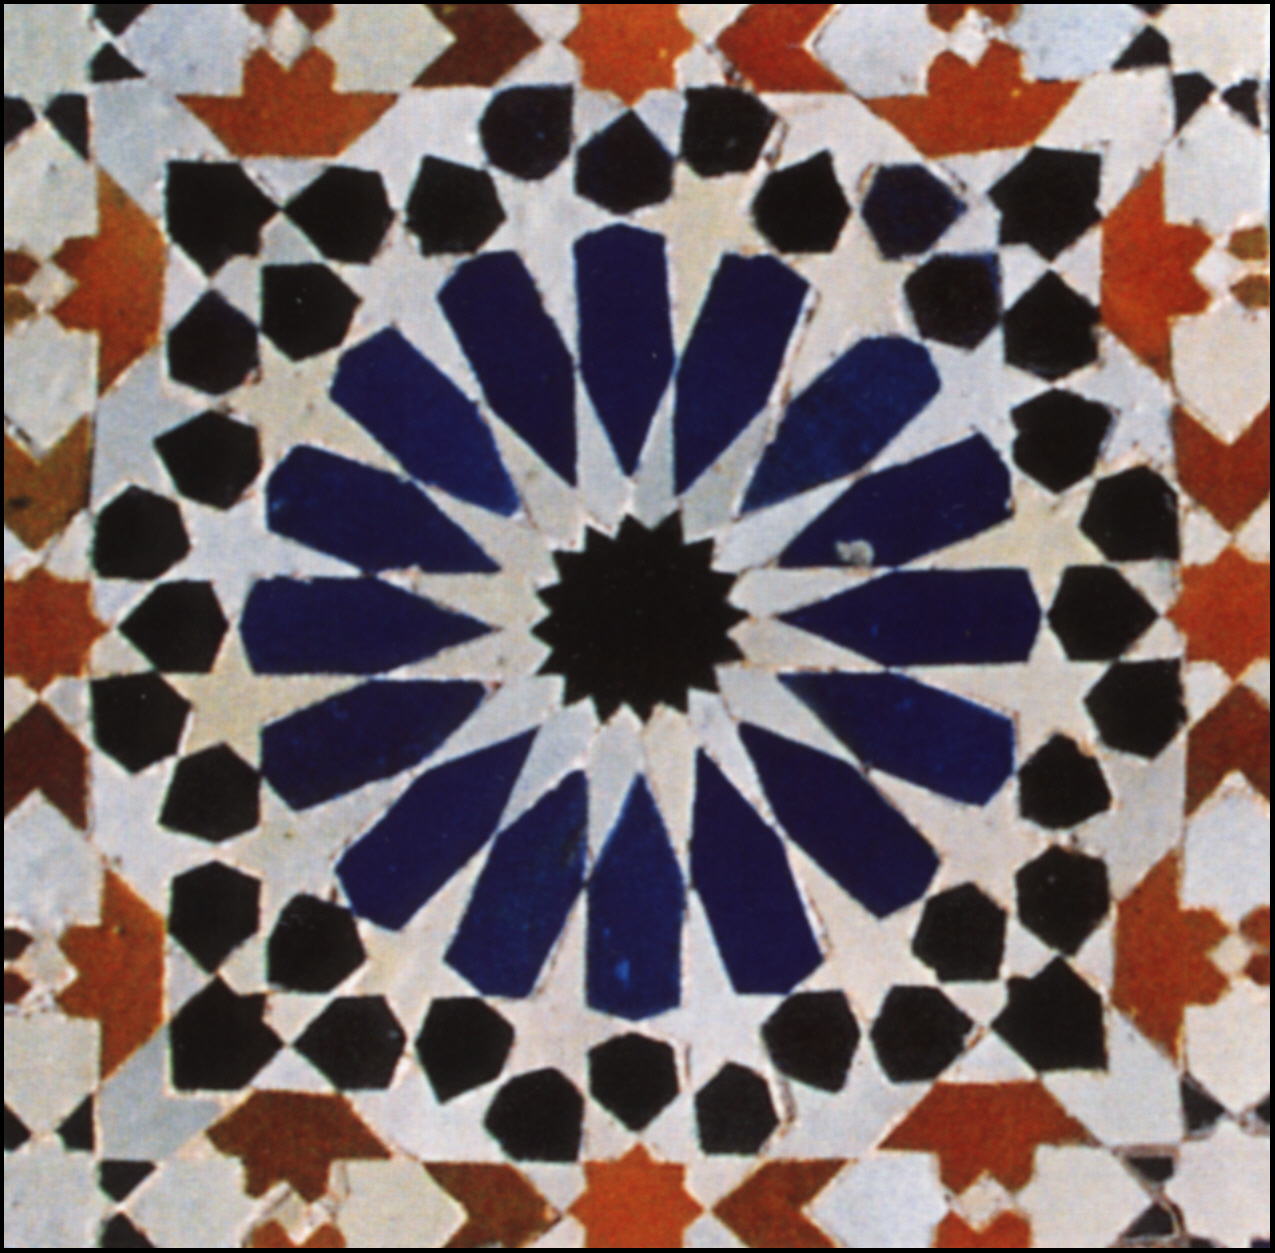
\includegraphics[width=\textwidth]{symetrie_motif_complet}
    \subcaption{Motif complet 
                \label{fig:sym_complet}}
  \end{minipage}
  \caption{Symétrie des motifs de zelliges \autocite{Castera_1996}.}
  \label{fig:symetrie}
\end{figure}

\section{Données physico-chimiques}
%----------------------------------------------------------------------

Les recherches bibliographiques préliminaires à l'étude au laboratoire 
ont permis de mettre en relief le manque de données physico-chimiques 
sur les zelliges.

Cependant, les zelliges sont en fait des pièces de céramique glaçurée, 
matériau étudié depuis de nombreuses années au CRPAA ainsi que dans 
d'autres laboratoires, et ayant fait l'objet de plusieurs publications 
% \autocite{Schvoerer_1998 ; Delvert_1991} 
et thèses 
\autocite{Rafaillac_1994}.

\chapter{Objectifs}
%======================================================================

Nous nous sommes fixé comme objectif principal pour cette étude, la 
recherche des technologies de fabrication anciennes. Ceci passe par 
une caractérisation physico-chimique de la céramique glaçurée. Elle 
se décompose en :

\begin{itemize}
\item La détermination des agents chromogènes responsables de la 
      couleur de la glaçure ;
\item Le calcul des coordonnées trichromatiques (qui donnent une 
      mesure objective de la couleur) ;
\item L'étude de la texture de la glaçure et du support céramique ;
\item La détermination des compositions élémentaires (glaçure et 
      terre cuite) ;
\item La détermination de la composition cristallographique de la 
      terre cuite.
\end{itemize}

Un deuxième objectif important est l'évaluation de l'état de 
conservation des échantillons et, le cas échéant, l'étude de leur 
altération.

Il sera également intéressant de réaliser une étude comparative 
entre les différents travaux menés en parallèle sur les zelliges au 
laboratoire, pour essayer d'en tirer des indices sur l'évolution 
chronologique et les différences géographiques de la technique des 
zelliges.

Enfin, les zelliges étant un sujet nouveau au laboratoire, il est 
particulièrement important de mettre en place une base de données, 
tant bibliographique que physico-chimique, sur ce matériau.
